\chapter{Umsetzung}\label{chap:umsetzung}

In diesem Kapitel wird eine mögliche parallelisierte Implementierung des \gls{fdk} vorgestellt. Dazu wird im ersten
Abschnitt ein Variantenvergleich vorgenommen, an den sich im zweiten Abschnitt die konkrete Implementierung anschließt.

\section{Variantenvergleich}

Dieser Abschnitt befasst sich mit dem Variantenvergleich verschiedener denkbarer Parallelisierungsstrategien. Zunächst
werden einige Ansätze aus der Literatur besprochen, die im Hinblick auf die Parallelisierung mit \gls{gpu}s von
besonderem Interesse sind, sowie auf deren Schwächen eingegangen. Danach wird das allen denkbaren Ansätzen
gemeine Problem des begrenzten \gls{gpu}-Speichers erläutert, woran sich dessen Abschwächung durch den Einsatz mehrerer
\gls{gpu}s anschließt.

\subsection{Bestehende Parallelisierungsstrategien und ihre Grenzen}\label{ssec:par_strat}

Von den in Abschnitt~\ref{ssec:par} genannten Ansätzen in der Literatur sind aufgrund ihrer Umsetzung für \gls{gpu}s die
Strategien von Xu et al. (vgl.~\cite{xumuell}), Scherl et al. (vgl.~\cite{scherlkeck}) und Zhao et al.
(vgl.~\cite{zhao}) von besonderem Interesse für diese Arbeit.

Da Xu et al. 2004 mit ihrer Arbeit Neuland betraten, standen ihnen viele Methoden und Technologien, die seitdem 
entwickelt wurden, noch nicht zur Verfügung. Die 2004 erschienenen \gls{gpu}s hatten im Vergleich zu heutigen
Grafikkarten sehr viel weniger Speicher; das damals beste verfügbare Produkt von NVIDIA{\textregistered}, die
GeForce{\textregistered} 6800 Ultra, konnte lediglich mit 512 MiB Speicher aufwarten und war nur über \gls{opengl} oder
\gls{directx} indirekt programmierbar (vgl.~\cite{geforce6800}). Den begrenzten Speicher versuchte die Gruppe durch eine
Aufteilung des Volumens und eine schichtweise Rekonstruktion desselben unter Einbeziehung aller Projektionen möglichst
effizient zu nutzen (vgl.~\cite{xumuell}). Aufgrund des technischen Fortschritts stehen uns heute andere Möglichkeiten
zur Lösung dieses Problems offen; so bietet etwa die NVIDIA{\textregistered} GeForce{\textregistered} GTX 1080 mit 8 GiB
Speicher und der Möglichkeit der direkten Programmierung mittels \gls{cuda} oder \gls{opencl} ganz andere Nutzungs- und
Berechnungsmöglichkeiten als ihre frühen Vorgänger (vgl.~\cite{gtx1080}). Insbesondere ist es möglich, das ganze Volumen
oder größere Teile davon während der Berechnung im Speicher zu halten und dadurch häufige Kopien zwischen
\gls{cpu}-Speicher und \gls{gpu}-Speicher zu vermeiden.

Die Forschungsgruppe um Scherl baute auf der Idee, das Volumen im Speicher zu halten, auf und ging im Gegensatz zu Xu et
al.\ den Weg, jede Projektion einzeln in dieses Volumen zu projizieren (vgl.~\cite{scherlkeck}). Zur Trennung bzw.\
Kapselung der einzelnen Schritte entwickelten sie in einem vorherigen Schritt (vgl.~\cite{scherlhopp}) eine
Pipeline-Struktur (nach Mattson et al., vgl.~\cite{mattsan}). Jeder Schritt des \gls{fdk} wird dabei in einer eigenen
Stufe (\textit{stage}) ausgeführt, die in einem separaten Thread ausgeführt wird. Zur Kommunikation der Ergebnisse der
einzelnen Stufen werden thread-sichere Puffer verwendet, auf die die Eingabe- bzw.\ Ausgaberoutinen der Stufen
zugreifen. Die eigentliche Rekonstruktion erfolgt entlang der $z$-Achse und der $y$-Achse: Jede $z$-Schicht im Volumen
wird entlang der $x$-Achse nocheinmal in Spalten aufgeteilt. Ein zweidimensionaler \gls{kernel} iteriert dann über alle
\gls{voxel} in $y$-Richtung (vgl. Abbildung~\ref{fig:scherl}). Der Nachteil des von Scherl et al.\ gewählten Ansatzes
liegt in der Pipeline-Struktur, die durch die wesentlich längere Laufzeit der Rückprojektion nicht optimal ist. So
schreiben Mattson et al.: {\glqq}If the stages in the pipeline vary widely in computational effort, the slowest stage
creates a bottleneck for the aggregate throughput{\grqq} (\cite{mattsan}, S. 106).

Die Grenzen bei dem vorgeschlagenen Verfahren der Gruppe um Zhao et al.\ sind vor allem praktischer Natur. Das von ihnen
vorgestellte Modell sieht vor, Symmetrien auszunutzen und dadurch Rechenzeit einzusparen (vgl.\
Abbildung~\ref{fig:zhao}). Sie machen sich dabei den Umstand zunutze, dass die auf den Detektor projizierte Koordinate
eines \gls{voxel}s der um 90 Grad rotierten Projektionskoordinate des um den gleichen Betrag rotierten Voxels
entspricht. Auf diese Weise lassen sich durch eine Berechnung die Detektorkoordinaten von vier \gls{voxel}n finden, was
eine Verkürzung der Rechenzeit verspricht (vgl.~\cite{zhao}). In der Praxis scheitert dieses Verfahren an dem
mechanischen Aufbau üblicher CT-Scanner. Da entweder Quelle und Detektor oder aber das Untersuchungsobjekt rotiert
werden müssen, kommt es durch Fehler in der Mechanik häufig dazu, dass Aufnahmen doppelt gemacht oder übersprungen
werden; auch kann es passieren, dass die Winkelschritte zwischen zwei Aufnahmen nicht immer einheitlich sind.

\begin{figure}[!htb]
    \centering
    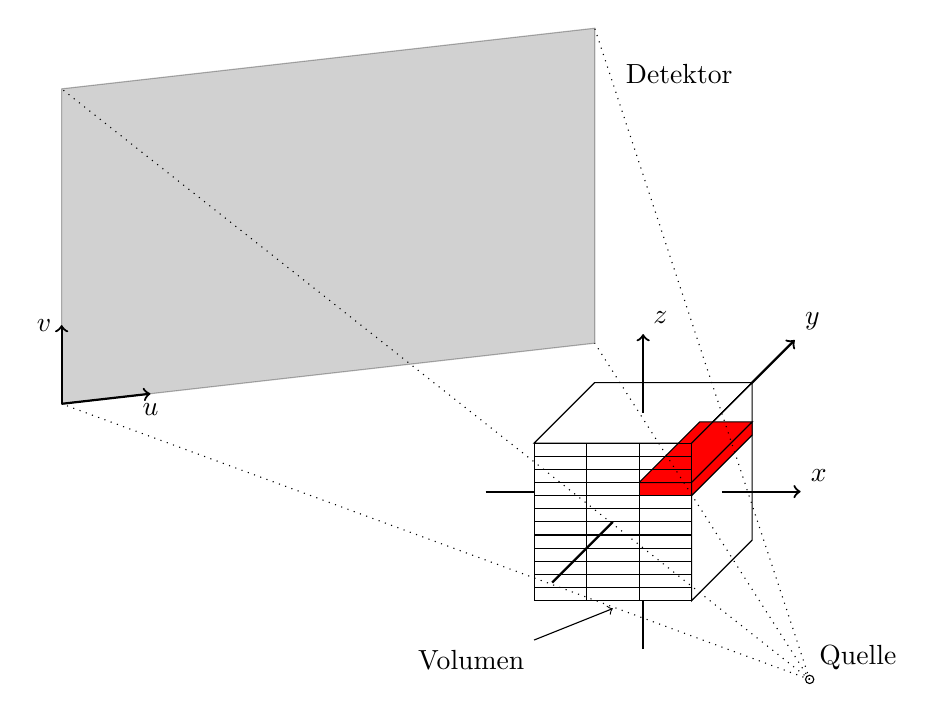
\begin{tikzpicture}[axis/.style={thick,->}]
        \draw[fill=black!60!white,opacity=0.3] (0, 0, 0) -- (0, 4, 0) -- (6, 4, -2) -- (6, 0, -2) -- (0, 0, 0);
        \draw[axis] (0, 0, 0) -- (0, 1, 0) node[left] {$v$};
        \draw[axis] (0, 0, 0) -- (1, 0, -0.33333333) node[below] {$u$};

        % Achsenanfang
        \draw[thick] (5, -1.5, -1) -- (6, -1.5, -1); % x
        \draw[axis] (7, -1.5, -2) -- (7, -1.5, -6) node[above right] {$y$}; % y
        \draw[thick] (7, -3.5, -1) -- (7, -2.5, -1); % z

        % Volumen
        \draw[fill=white] (6, -0.5, -2) -- (8, -0.5, -2) -- (8, -0.5, 0) -- (6, -0.5, 0) -- (6, -0.5, -2);
        \draw[fill=white] (6, -0.5, 0) -- (8, -0.5, 0) -- (8, -2.5, 0) -- (6, -2.5, 0) -- (6, -0.5, 0);
        \draw[fill=white] (8, -0.5, -2) -- (8, -2.5, -2) -- (8, -2.5, 0) -- (8, -0.5, 0) -- (8, -0.5, -2);

        \draw[->] (6, -3, 0) -- (7, -2.6, 0) node[pos=0,below left] {Volumen};

        % Achsenende
        \draw[axis] (8, -1.5, -1) -- (9, -1.5, -1) node[above right] {$x$}; % x
        \draw[thick] (7, -1.5, 2) -- (7, -1.5, 0); % y
        \draw[axis] (7, -0.5, -1) -- (7, 0.5, -1) node[above right] {$z$}; % z

        % Teilvolumen
        \draw[fill=red] (7.333333, -1, 0) -- (8, -1, 0) -- (8, -1.166666, 0) -- (7.333333, -1.166666, 0)
                        -- (7.333333, -1, 0);
        \draw[fill=red] (7.333333, -1, 0) -- (7.333333, -1, -2) -- (8, -1, -2) -- (8, -1, 0) -- (7.333333, -1, 0);
        \draw[fill=red] (8, -1, 0) -- (8, -1, -2) -- (8, -1.166666, -2) -- (8, -1.166666, 0) -- (8, -1, 0);

        \draw (6.666666, -0.5, 0) -- (6.666666, -2.5, 0); % v1
        \draw (7.333333, -0.5, 0) -- (7.333333, -2.5, 0); % v2
        \draw (6, -0.666666, 0) -- (8, -0.666666, 0); % h1
        \draw (6, -0.833333, 0) -- (8, -0.833333, 0); % h2
        \draw (6, -1, 0) -- (8, -1, 0); % h3
        \draw (6, -1.166666, 0) -- (8, -1.166666, 0); % h4
        \draw (6, -1.333333, 0) -- (8, -1.333333, 0); % h5
        \draw (6, -1.5, 0) -- (8, -1.5, 0); % h6
        \draw (6, -1.666666, 0) -- (8, -1.666666, 0); % h7
        \draw (6, -1.833333, 0) -- (8, -1.833333, 0); % h8
        \draw (6, -2, 0) -- (8, -2, 0); % h9
        \draw (6, -2.166666, 0) -- (8, -2.166666, 0); % h10
        \draw (6, -2.333333, 0) -- (8, -2.333333, 0); % h11

        % fehlende Linien nachzeichnen
        \draw (8, -0.5, 0) -- (8, -0.5, -2);
        \draw (8, -0.5, 0) -- (8, -2.5, 0);
        \draw (6, -0.5, 0) -- (8, -0.5, 0);

        % Quelle und Kegelstrahl
        \coordinate (s) at (9.5, -3.5, 0);
        \draw (s) circle (1.5pt) node[above right] {Quelle};
        \draw[dotted] (s) -- (0, 0, 0);
        \draw[dotted] (s) -- (0, 4, 0);
        \draw[dotted] (s) -- (6, 4, -2) node[pos=0.9,above right] {Detektor};
        \draw[dotted] (s) -- (6, 0, -2);
    \end{tikzpicture}
    \captionof{figure}{Aufteilung des Volumens nach Scherl et al. (Vorlage:~\cite{scherlkeck})}
    \label{fig:scherl}
\end{figure}

\begin{figure}[!htb]
    \centering
    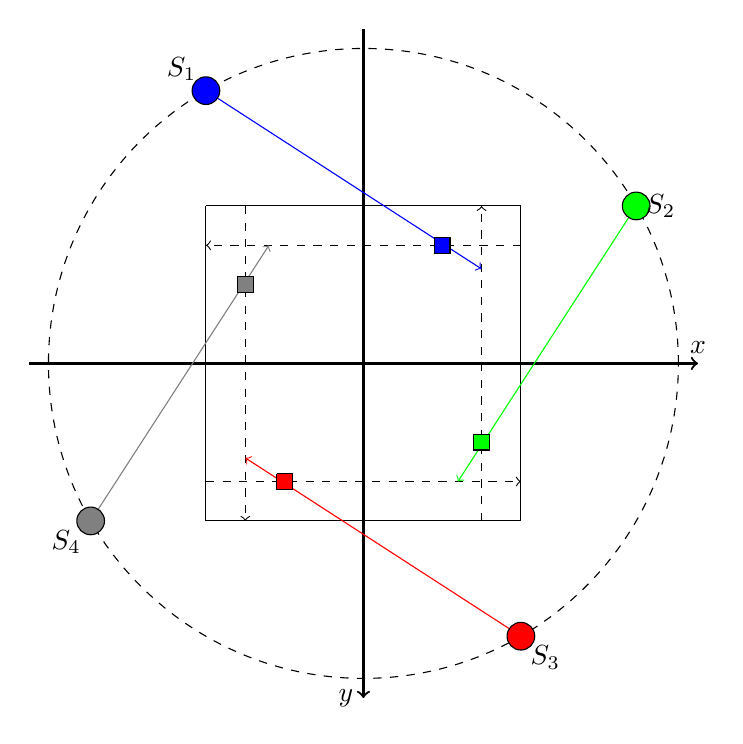
\begin{tikzpicture}[axis/.style={thick,->}]
        \draw[axis] (0, 4.25, 0) -- (0, -4.25, 0) node [left] {$y$};
        \draw[axis] (-4.25, 0, 0) -- (4.25, 0, 0) node [above] {$x$};

        % Volumen
        \draw (-2, 2, 0) -- (2, 2, 0) -- (2, -2, 0) -- (-2, -2, 0) -- (-2, 2, 0);

        % Pfeile im Volumen
        \draw[dashed,->] (-1.5, 2, 0) -- (-1.5, -2, 0);
        \draw[dashed,->] (2, 1.5, 0) -- (-2, 1.5, 0);
        \draw[dashed,->] (1.5, -2, 0) -- (1.5, 2, 0);
        \draw[dashed,->] (-2, -1.5, 0) -- (2, -1.5, 0);

        % Kreis
        \draw[dashed] (0, 0, 0) circle [radius=4];

        % Quellpfeile
        \draw[color=blue,->] (-2, 3.46410) -- (1.5, 1.2);
        \draw[color=green,->] (3.46410, 2) -- (1.2, -1.5);
        \draw[color=red,->] (2, -3.46410) -- (-1.5, -1.2);
        \draw[color=gray,->] (-3.46410, -2) -- (-1.2, 1.5);

        % Quellpositionen
        \draw[fill=blue] (-2, 3.46410) circle (5pt) node [above left] {$S_1$};
        \draw[fill=green] (3.46410, 2) circle (5pt) node [right] {$S_2$};
        \draw[fill=red] (2, -3.46410) circle (5pt) node [below right] {$S_3$};
        \draw[fill=gray] (-3.46410, -2) circle (5pt) node [below left] {$S_4$};

        % Voxel
        \draw[fill=blue] (0.9, 1.6) -- (1.1, 1.6) -- (1.1, 1.4) -- (0.9, 1.4) -- (0.9, 1.6);
        \draw[fill=green] (1.4, -0.9) -- (1.6, -0.9) -- (1.6, -1.1) -- (1.4, -1.1) -- (1.4, -0.9);
        \draw[fill=red] (-1.1, -1.4) -- (-0.9, -1.4) -- (-0.9, -1.6) -- (-1.1, -1.6) -- (-1.1, -1.4);
        \draw[fill=gray] (-1.6, 1.1) -- (-1.4, 1.1) -- (-1.4, 0.9) -- (-1.6, 0.9) -- (-1.6, 1.1);
    \end{tikzpicture}
    \captionof{figure}{Symmetrien bei der Rückprojektion nach Zhao et al. (Vorlage:~\cite{zhao})}
    \label{fig:zhao}
\end{figure}

\subsection{Das Problem des GPU-Speichers}

Den oben vorgestellten Ansätzen ist gemein, dass sie alle mit dem limitierten Speicher einer \gls{gpu} arbeiten mussten.
Während der technische Fortschritt die Speichergrenze seitdem weiter nach oben verschoben hat, hat sich das
zugrundeliegende Problem dennoch nicht wesentlich verändert. Mit modernen \gls{gpu}s wie der NVIDIA{\textregistered}
GeForce{\textregistered} GTX 1080 ist es inzwischen zwar möglich, komplette Volumen oder wenigstens große Teile
davon während der Rückprojektion im \gls{gpu}-Speicher zu halten und so die Zahl der Kopien zwischen \gls{host} und
\gls{device} zu reduzieren; der parallel stattfindende Fortschritt bei der Computertomographie, insbesondere im
Hinblick auf die Detektorauflösung und die dadurch produzierte Datenmenge, erhöht allerdings auch weiterhin den für die
Berechnung erforderlichen Speicher. Im Gegensatz zu den klassischen \gls{cpu}s, deren Speicher sich theoretisch nahezu
unbegrenzt erhöhen lässt, ist für die Parallelisierung mit \gls{gpu}s eine Strategie zur Verwaltung des zur Verfügung
stehenden Speichers also weiterhin unabdingbar.

\subsection{Heterogene GPU-Systeme und effiziente Arbeitsteilung}

Ein naheliegender Weg zur Umgehung des begrenzten \gls{gpu}-Speichers ist der parallele Einsatz mehrerer \gls{gpu}s.
Dieser Ansatz wirft jedoch einige neue Probleme auf.

Am vordringlichsten ist die Frage zu beantworten, in welcher
Form die Berechnung auf die verfügbaren \gls{gpu}s verteilt werden soll. Während dies für den Fall, dass mehrere
gleichartige \gls{gpu}s verwendet werden sollen, relativ einfach ist, wird die Lastverteilung beim Einsatz
unterschiedlich leistungsstarker Grafikkarten deutlich schwieriger. Es ist zu vermeiden, dass die schnelleren \gls{gpu}s
auf die langsameren warten müssen, da so Rechenzeit verschenkt wird.

In beiden Fällen kommt hinzu, dass die vorhandenen Grafikkarten möglichst parallel mit Daten befüllt und zur Berechnung
gebracht werden sollen, die vorgesehenen Schritte der Rückprojektion also weitestgehend gleichzeitig ausgeführt werden.

\subsection{Lösungsvorschlag}\label{ssec:loesungsvorschlag}

Aus den oben genannten Faktoren beim Einsatz von \gls{gpu}s ergeben sich die folgenden Anforderungen an eine effiziente
Parallelisierungsstrategie des \gls{fdk}:

\begin{enumerate}
    \item der auf \gls{gpu}s beschränkte Speicher muss möglichst effizient genutzt werden, häufige Kopien sollten also
          vermieden werden.
    \item Die Optimierung der Rückprojektionen sollte die höchste Priorität genießen, woraus folgt, dass
    \item die Rückprojektion die zur Verfügung stehenden \gls{gpu}s möglichst stark auslasten sollte.
    \item Die Wartezeit zwischen zwei Rückprojektionen sollte möglichst minimal sein, also nicht auf die Wichtung und
          Filterung warten müssen.
    \item Die Parallelisierung sollte sich möglichst effizient über mehrere \gls{gpu}s skalieren lassen.
\end{enumerate}

Mit der Umsetzung der Punkte 2.\ und 3.\ beschäftigt sich detailliert der nächste Abschnitt, ein Lösungsvorschlag für
die restlichen Punkte findet sich in der im Folgenden skizzierten Programmstruktur.

Ein typischer Projektionsdatensatz umfasst 1440 Projektionen, die jeweils eine Auflösung von 1024 x 1024 \gls{pixel}n
haben; jeder Pixel ist dabei im 4-Byte-Fließkommazahlen-Format gespeichert. Für den kompletten Datensatz ergibt sich
dadurch eine Datenmenge von 5,625 GiB. Das daraus resultierende Volumen besitzt (abhängig von den konkreten
Geometrieparametern der CT-Anlage) etwa 1070 x 1070 x 1033 \gls{voxel} (vgl. Abschnitt~\ref{ssec:geometrie}), die das
gleiche Datenformat wie die Pixel aufweisen. Die Datengröße des Volumens beträgt 4,4 GiB und die kumulierte Datenmenge
damit 10,25 GiB. Ausgehend von der Annahme, dass eine \gls{gpu} des Typs GeForce{\textregistered} GTX 1080 zur Verfügung
steht, ist allein mit den zu verarbeitenden Daten der verfügbare \gls{gpu}-Speicher nicht ausreichend, da die GTX 1080
über lediglich 8 GiB Speicher verfügt (siehe~\cite{gtx1080}). Sowohl die Projektionen als auch das komplette Volumen im
Speicher zu halten ist demnach kein praktikabler Ansatz. In Abschnitt~\ref{ssec:par_strat} wurden mehrere Ansätze der
Literatur vorgestellt, die dieses Problem zu umgehen versuchen.

Der erste Ansatz von Xu et al.\ sieht eine Aufteilung des Volumens in mehrere Segmente vor. Jedes Teilvolumen wird dann
durch die Iteration über den kompletten Projektionsdatensatz berechnet (vgl.~\cite{xumuell}). Allerdings muss bei diesem
Ansatz zusätzlich zur Aufteilung des Volumens ein Weg gefunden werden, alle Projektionen effizient auf der \gls{gpu}
abzubilden, da -- wie oben gezeigt -- der Projektionsdatensatz tendenziell größer ist als das komplette Volumen. Dies
erzeugt zusätzliche Komplexität und damit unerwünschten \textit{overhead}.

Scherl et al.\ schlagen den umgekehrten Weg vor, sodass das ganze Volumen bzw.\ ein möglichst großer Teil davon im
Speicher gehalten wird. Die Projektionen werden dann einzeln geladen und in das Volumen zurückprojiziert
(vgl.~\cite{scherlkeck}). Gegenüber der von Xu et al.\ gewählten Variante bietet dies den Vorteil, dass nicht mehr alle
Projektionen im Speicher gehalten werden bzw.\ im richtigen Iterationsschritt vorhanden sein müssen; stattdessen werden
die Projektionen sequentiell geladen und verarbeitet. Im idealen Fall (das ganze Volumen passt in den Speicher) entfällt
zudem die Notwendigkeit für Teilvolumen, sodass es genau einen Kopiervorgang bezüglich des Volumens am Ende der
Berechnung gibt.

Für den Fall, dass das Volumen nicht in Gänze in den \gls{gpu}-Speicher passt, schlagen Zhao et al.\ eine Aufteilung
entlang der $z$-Achse vor (vgl.~\cite{zhao}). Das Volumen wird dabei in $N$ gleich große Teilvolumen zerlegt, die
einzeln in den \gls{gpu}-Speicher passen. Jede Projektion wird dann ebenfalls in $N$ Teilprojektionen unterteilt, sodass
jede Teilprojektion geometrisch einem Teilvolumen entspricht. Dieser Ansatz hat jedoch den Nachteil, dass die für das
aktuell zu rekonstruierende Teilvolumen nicht benötigten Teilprojektionen verwaltet bzw.\ zwischengespeichert werden
müssen, was ebenfalls zusätzliche Komplexität in den Algorithmus einführt.

Aufgrund der geschilderten Vorteile im Hinblick auf den begrenzt verfügbaren \gls{gpu}-Speicher ist es daher sinnvoll,
dem Ansatz von Scherl et al.\ zu folgen und die Rückprojektion sequentiell für jede Projektion durchzuführen, während
das ganze Volumen im Speicher gehalten wird. Sollte der vorhandene Speicher nicht ausreichen, muss das Volumen
in mehrere Teilvolumen zerlegt werden, die dann einzeln rekonstruiert und zum Schluss wieder zusammengesetzt werden.
Abweichend von Zhao et al.\ ist eine entsprechende Unterteilung der Projektionen aus zweierlei Gründen nicht notwendig.
Einerseits besitzt eine einzelne Projektion des obigen Beispiels eine im Vergleich zum Volumen vernachlässigbare
Datengröße von 4 MiB, sodass der durch eine Aufteilung eingesparte Speicher keinen nennenswerten Mehrwert bietet,
andererseits ist der Zeitaufwand der Wichtungs- und Filteroperationen verglichen mit der Rückprojektion derart gering,
dass die Durchführung dieser Operationen auf weniger Pixeln in Bezug auf die Gesamtlaufzeit keine bemerkenswerte
Zeitersparnis verspricht. Es ist hierbei zu beachten, dass dadurch alle Projektionen für jedes Teilvolumen neu geladen
werden müssen, sobald die Berechnung des vorherigen Teilvolumens abgeschlossen ist. Bei einer Datenübertragung über das
Netzwerk oder einer langsamen Festplatte kann sich dieser Faktor schnell zu einem Flaschenhals entwickeln, sofern der
(gegebenenfalls gewichtete und gefilterte) Projektionsdatensatz nicht auf andere Art und Weise zwischengespeichert
werden kann.

Eine weitere Herausforderung ist die Minimierung der Wartezeit zwischen zwei aufeinanderfolgenden Rückprojektionen.
Theoretisch wäre es hier denkbar, zwei oder mehr Rückprojektionen verschiedener Projektionen gleichzeitig durchzuführen.
Praktisch ergäbe sich daraus die Notwendigkeit der Synchronisierung zwischen den verschiedenen
Rückprojektionsoperationen, um Datenkorruption durch \textit{\glspl{race-condition}} zu vermeiden. Es ist daher der
einfachere Weg, die Rückprojektionen in sequentieller Reihenfolge durchzuführen. Um die Wartezeiten zwischen zwei
Rückprojektionen zu minimieren, sollten möglichst keine weiteren Operationen in der Zwischenzeit ausgeführt werden.
Idealerweise werden dann -- neben dem der Rückprojektion -- nur noch das Entnehmen der aktuellen Projektion vom
Eingabepuffer sowie das Übergeben dieser Projektion an den Rückprojektions-\gls{kernel} ausgeführt. Demzufolge muss die
beschriebene Ausführungskette in einem eigenen Thread ausgeführt werden, um die restlichen Operationen, insbesondere die
Wichtung und die Filterung der Projektionen, durch Nebenläufigkeiten zu kaschieren.

Schwieriger ist eine effiziente Skalierung des \gls{fdk} auf heterogenen \gls{gpu}-Systemen, also Systemen mit
unterschiedlich leistungsstarken Grafikkarten. In der Literatur gibt es in jüngerer Zeit Ansätze zur besseren
(nicht FDK-spezifischen) Lastverteilung durch den Einsatz von \textit{machine-learning}-Techniken (vgl.~\cite{linhsi}),
eine Implementierung eines solchen Verfahrens geht allerdings über den Fokus dieser Arbeit hinaus und bedarf daher einer
gesonderten Untersuchung. Für den Fall, dass der implementierte Algorithmus auf einem System mit mehreren \gls{gpu}s zum
Einsatz kommt, wird daher die zu erledigende Arbeit statisch über alle verfügbaren \gls{gpu}s verteilt. Zunächst wird
das Gesamtvolumen in $N$ gleich große Teilvolumen zerlegt, wobei $N$ die Zahl der im System vorhandenen \gls{gpu}s
bezeichnet. Ist die Zahl der Schichten im Gesamtvolumen nicht glatt durch $N$ teilbar, wird der Rest an das unterste
Teilvolumen angehängt. Im Anschluss daran wird überprüft, ob diese Teilvolumen gemeinsam mit ein wenig zusätzlichem
Puffer für Projektions- und Berechnungsdaten in den kleinsten vorhandenen \gls{gpu}-Speicher passen. Ist dies nicht der
Fall, werden alle Teilvolumen so lange durch zwei geteilt, bis die so entstandenen kleineren Teilvolumen klein genug für
den Speicher sind. Für jede vorhandene Grafikkarte wird dann ein separater Thread gestartet, der die Schritte
\textit{Projektion laden} -- \textit{Wichtung} -- \textit{Filterung} -- \textit{Rückprojektion} auf dieser \gls{gpu}
ausführt (siehe Quelltext~\ref{source:high_level_fdk}). Hierbei ist zu beachten, dass aufgrund der oben geschilderten
Vorgehensweise zur Reduktion der Wartezeiten die Rückprojektion nochmals in einem weiteren Thread läuft, sodass die
Anzahl der insgesamt gestarteten Threads $2 \cdot N$ beträgt.

\begin{code}
\begin{minted}[breaklines,breakafter=\,,fontsize=\small]{c++}
// Diese Funktion läuft in einem separaten Thread pro GPU
auto fdk(task_queue& queue, // enthält ausstehende Teilvolumen
         int device) -> void
{
    cudaSetDevice(device);

    while(!queue.empty()) // solange es unbearbeitete Teilvolumen gibt
    {
        auto t = queue.pop(); // hole Teilvolumen-Informationen
        auto s = source(...); // konfiguriere Laden der Projektionen

        auto v = make_volume(...); // erzeuge Teilvolumen auf Device

        while(!source.drained()) // für jede Projektion
        {
            auto p = source.load_next(); // lade nächste Projektion
            auto d_p = copy_h2d(p); // kopiere Projektion auf Device
            weight(d_p, ...); // wichte Projektion
            filter(d_p, ...); // filtere Projektion

            /* Rückprojektion. Startet intern einen weiteren Thread,
               der die übergebenen Projektionen weiter verarbeitet */
            backproject(d_p, v, ...);
        }

        save_subvolume(v, ...); // Teilvolumen abspeichern
    }
}     
\end{minted}
\captionof{listing}{Funktionsabfolge des implementierten FDK-Algorithmus}
\label{source:high_level_fdk}
\end{code}

\section{Implementierung und Optimierung}

In diesem Abschnitt werden die Implementierung und die Optimierung des \gls{fdk} beschrieben. Zunächst werden die
Implementierungs- und Optimierungsziele sowie die Einflüsse der realen Welt auf das Modell vorgestellt und im Anschluss
daran die Umsetzung der Stufen \textit{Wichtung} und \textit{Filterung} gezeigt. Der Abschnitt schließt mit der
Implementierung der Rückprojektion.

\subsection{Implementierungs- und Optimierungsziele}

Von den in Abschnitt~\ref{ssec:loesungsvorschlag} genannten Zielen einer Implementierung des \gls{fdk} sind im Hinblick
auf die Nutzung von \gls{cuda} die zusammenhängenden Faktoren \textit{Optimierung} und \textit{\gls{gpu}-Auslastung}
von großer Bedeutung. Da die Rückprojektion im Vergleich zur Wichtung und Filterung einen weitaus höheren Rechenaufwand
erfordert, ist ihrer Optimierung die höchste Priorität einzuräumen, sodass der gesamte Algorithmus für derzeit gängige
Datensätze der Computertomographie -- also bis zu einer Projektionsauflösung von 1024 x 1024 \gls{pixel}n -- auf neuer
Hardware in wenigen Minuten lösbar ist. Da die \gls{cuda}-Plattform den parallelen Einsatz mehrerer \gls{gpu}s
unterstützt, ist die Implementierung so zu konzipieren, dass sie auf einer oder mehreren Grafikkarten korrekte
Ergebnisse bei gleichzeitiger Beschleunigung des Gesamtalgorithmus berechnet.

\subsection{Optimierungsüberlegungen}\label{ssec:opti_ueber}

Die Optimierung eines \gls{kernel}s fußt im Wesentlichen auf drei Dingen:

\begin{enumerate}
    \item Die Auslastung der Grafikkarte muss möglichst hoch sein, um die vorhandenen Rechenkapazitäten effektiv nutzen
          zu können. Bedingung für eine effektive Verteilung des \gls{kernel}s ist ein möglichst geringer
          Registerverbrauch innerhalb eines \gls{sm}s, sodass die maximale Zahl an Kernen genutzt werden kann.
    \item Die Zeit zwischen zwei \gls{kernel}-Aufrufen muss minimiert werden, um die Gesamtrechenzeit zu verkürzen.
    \item Die langsamen Zugriffe auf den globalen Speicher müssen möglichst effizient sein, um den Algorithmus nicht
          auszubremsen.
\end{enumerate}

Da, wie wir gesehen haben, die gefilterte Rückprojektion von einer Reihe geometrischer Parameter abhängt, ist die Zahl
der benötigten Register für die Übergabe dieser Parameter sowie zur Speicherung von Zwischenergebnissen potentiell hoch.
Ein großer Teil dieser Parameter ist jedoch für die (teils komplette, teils projektionsweise) Rückprojektion konstant,
wie zum Beispiel die Abstände zwischen dem Objekt, der Quelle und dem Detektor oder die geometrischen Eigenschaften
des Detektors. Da sich diese Parameter auch während der Berechnung nicht ändern können, empfiehlt es sich, diese in
den konstanten Speicher der Grafikkarte auszulagern, auf den verhältnismäßig schnell zugegriffen werden kann.

Anders verhält es sich mit den Projektionen und dem Volumen. Da während der Ausführung auf beide Speicherbereiche
schreibend zugegriffen werden muss, ist es sinnvoll, diese Zugriffe möglichst optimal zu gestalten. Da die Projektionen
der Kegelstrahltomographie üblicherweise zweidimensional sind und das zu rekonstruierende Volumen dreidimensional ist,
können die für zwei- bzw.\ dreidimensionale Operationen optimierten Speichervarianten der \gls{cuda}-Plattform verwendet
werden, die man mit \texttt{cudaMallocPitch} bzw.\ \texttt{cudaMalloc3D} alloziiert. Zusätzlich ist es nach der Wichtung
und der Filterung für die Rückprojektion nicht mehr erforderlich, die Projektionen zu verändern. Durch deren Umwandlung
in Texturen bzw.\ deren Verschiebung in den für Texturzugriffe optimierten Teil des globalen Speichers, der einen
speziellen Cache besitzt, kann der Zeitverlust beim lesenden Zugriff auf die Projektionen minimiert werden.

Die Verringerung der Zeit zwischen zwei \gls{kernel}-Ausführungen dient der Verkürzung der gesamten Rechenzeit.

\subsection{Einflüsse der realen Welt}

Die in Kapitel~\ref{chap:grundlagen} gezeigten Überlegungen zur gefilterten Rückprojektion und dem \gls{fdk} sind in
dieser Form rein theoretischer Natur. Die Anwendung dieser Modelle auf die reale Welt ist mit einigen Schwierigkeiten
bzw.\ Einflüssen verbunden, die im Folgenden näher vorgestellt werden sollen.

\subsubsection{Detektorgeometrie}

Der Detektor übt aufgrund der durch ihn gewonnenen Informationen (in Form der Projektionen) einen großen Einfluss auf
die gefilterte Rückprojektion aus. Seinem Aufbau muss daher bei der Implementierung des \gls{fdk} besondere
Aufmerksamkeit zukommen.

Der Detektor hat eine feste Breite und Höhe (gemessen in Millimetern) und besteht aus einer zweidimensionalen Anordnung
von \gls{pixel}n (siehe Abbildung~\ref{fig:det_geometrie}). In der horizontalen Richtung verfügt er über $N_h$
\gls{pixel}, in der vertikalen Richtung sind es $N_v$ \gls{pixel}.

Jedes \gls{pixel} hat eine physische Breite $d_h$ und Höhe $d_v$ (gemessen in Millimetern); äquivalent lassen sich diese
Ausdehnungen als horizontale (vertikale) Abstände zwischen den \gls{pixel}zentren betrachten (siehe
Abbildung~\ref{fig:det_pixel}).

Spannt man nun über dem Detektor ein Koordinatensystem auf (mit dessen Zentrum als Ursprung, siehe
Abbildung~\ref{fig:det_koord}), wobei $h_{min}$, $h_{max}$, $v_{min}$ und $v_{max}$ den horizontalen (vertikalen)
Abstand von den Detektorrändern bis zur Detektormitte in Millimetern angeben, so ergeben sich die folgenden
Zusammenhänge:

\begin{equation}\label{eq:det_h}
    \begin{aligned}
        h_{max} - h_{min} &= N_h \cdot d_h\\
        h_{min} + \frac{N_h \cdot d_h}{2} &= 0
    \end{aligned}
\end{equation}

\begin{equation}\label{eq:det_v}
    \begin{aligned}
        v_{max} - v_{min} &= N_v \cdot d_v\\
        v_{min} + \frac{N_v \cdot d_v}{2} &= 0
    \end{aligned}
\end{equation}

\begin{figure}[!tb]
    \centering
    \begin{minipage}[b]{.5\textwidth}
        \centering
        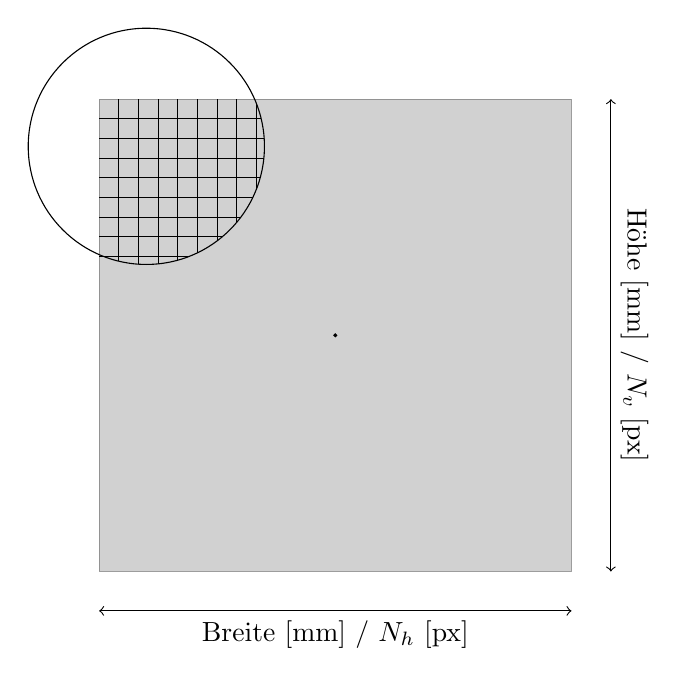
\begin{tikzpicture}
            \draw[fill=black!60!white,opacity=0.3] (-3, 3) -- (3, 3) -- (3, -3) -- (-3, -3) -- (-3, 3);
            \draw[fill=black] (0,0) circle (0.5pt);

            % Lupe
            \draw (-2.4, 2.4) circle (1.5cm);

            % Pixellinien vertikal
            \draw (-2.75, 3) -- (-2.75, 0.95);
            \draw (-2.5, 3) -- (-2.5, 0.9);
            \draw (-2.25, 3) -- (-2.25, 0.9);
            \draw (-2, 3) -- (-2, 0.95);
            \draw (-1.75, 3) -- (-1.75, 1.05);
            \draw (-1.5, 3) -- (-1.5, 1.2);
            \draw (-1.25, 3) -- (-1.25, 1.43);
            \draw (-1, 2.94) -- (-1, 1.85);

            % Pixellinien horizontal
            \draw (-3, 2.75) -- (-0.95, 2.75);
            \draw (-3, 2.5) -- (-0.9, 2.5);
            \draw (-3, 2.25) -- (-0.9, 2.25);
            \draw (-3, 2) -- (-0.95, 2);
            \draw (-3, 1.75) -- (-1.05, 1.75);
            \draw (-3, 1.5) -- (-1.2, 1.5);
            \draw (-3, 1.25) -- (-1.43, 1.25);
            \draw (-3, 1) -- (-1.85, 1);

            % Pfeile und Beschriftungen
            \draw[<->] (-3, -3.5) -- (3, -3.5) node[pos=0.5, below] {Breite [mm] / $N_h$ [px]};
            \draw[<->] (3.5, 3) -- (3.5, -3) node[pos=0.5, sloped, above] {Höhe [mm] / $N_v$ [px]};
        \end{tikzpicture}
        \captionof{figure}{Detektorgeometrie}
        \label{fig:det_geometrie}
    \end{minipage}%
    \begin{minipage}[b]{.5\textwidth}
        \centering
        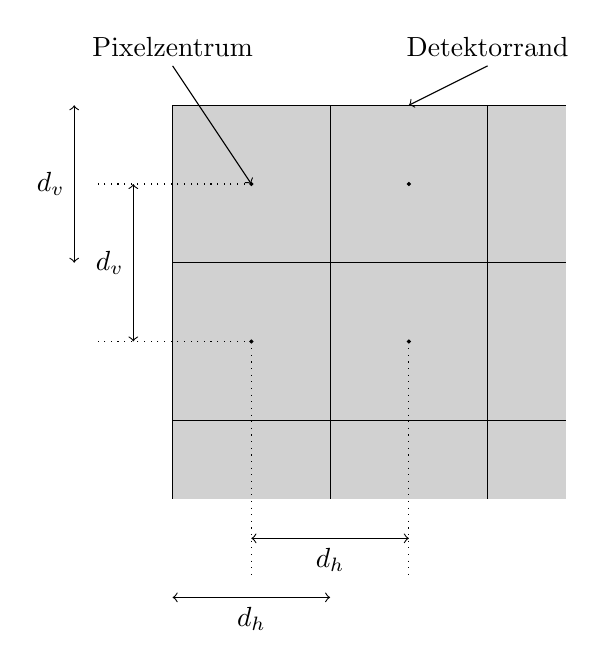
\begin{tikzpicture}
            \fill[black!60!white,opacity=0.3] (-2, 2) rectangle (3, -3);
            \draw (-2, 2) -- (2, 2) -- (2, -2) -- (-2, -2) -- (-2, 2);
            \draw (2, 2) -- (3, 2);
            \draw (-2, 0) -- (3, 0);
            \draw (0, 2) -- (0, -3);
            \draw (-2, 2) -- (-2, -3);
            \draw (2, -2) -- (2, -3);
            \draw (2, -2) -- (3, -2);
            \draw[fill=black] (-1, 1) circle (0.5pt);
            \draw[fill=black] (1, 1) circle (0.5pt);
            \draw[fill=black] (1, -1) circle (0.5pt);
            \draw[fill=black] (-1, -1) circle (0.5pt);

            % Verlängerungen
            \draw[dotted] (-1, 1) -- (-3, 1);
            \draw[dotted] (-1, -1) -- (-3, -1);
            \draw[dotted] (-1, -1) -- (-1, -4);
            \draw[dotted] (1, -1) -- (1, -4);

            % Pfeile und Beschriftungen
            \draw[->] (2, 2.5) -- (1, 2) node[pos=0, above] {Detektorrand};
            \draw[->] (-2, 2.5) -- (-1, 1) node[pos=0, above] {Pixelzentrum};
            \draw[<->] (-2.5, 1) -- (-2.5, -1) node[pos=0.5, left] {$d_v$};
            \draw[<->] (-3.25, 2) -- (-3.25, 0) node[pos=0.5, left] {$d_v$};
            \draw[<->] (-1, -3.5) -- (1, -3.5) node[pos=0.5, below] {$d_h$};
            \draw[<->] (-2, -4.25) -- (0, -4.25) node[pos=0.5, below] {$d_h$};
        \end{tikzpicture}
        \captionof{figure}{Pixelgeometrie}
        \label{fig:det_pixel}
    \end{minipage}
\end{figure}

\begin{figure}[!tb]
    \centering
    \begin{minipage}[b]{.5\textwidth}
        \centering
        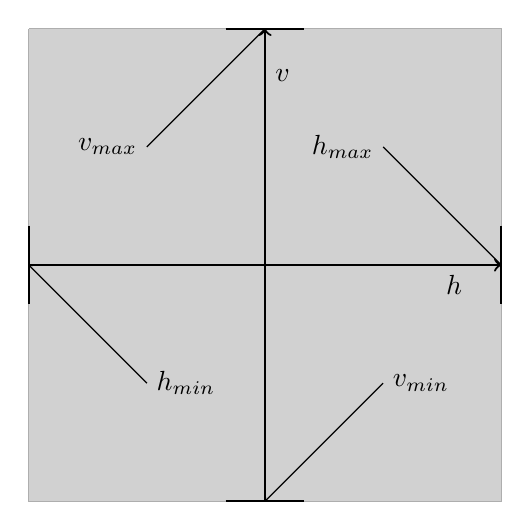
\begin{tikzpicture}[axis/.style={thick,->}]
            \draw[fill=black!60!white,opacity=0.3] (-3, 3) -- (3, 3) -- (3, -3) -- (-3, -3) -- (-3, 3);
            \draw[fill=black] (0,0) circle (0.5pt);

            % Achsen
            \draw[axis] (0, -3) -- (0, 3) node [pos=0.9, right] {$v$};
            \draw[axis] (-3, 0) -- (3, 0) node [pos=0.9, below] {$h$};

            % Markierungen
            \draw[thick] (-3, 0.5) -- (-3, -0.5);
            \draw[thick] (3, 0.5) -- (3, -0.5);
            \draw[thick] (-0.5, 3) -- (0.5, 3);
            \draw[thick] (-0.5, -3) -- (0.5, -3);

            % Beschriftungen
            \draw[->] (1.5, 1.5) -- (3, 0) node [pos=0, left] {$h_{max}$};
            \draw[->] (-1.5, -1.5) -- (-3, 0) node [pos=0, right] {$h_{min}$};
            \draw[->] (-1.5, 1.5) -- (0, 3) node [pos=0, left] {$v_{max}$};
            \draw[->] (1.5, -1.5) -- (0, -3) node [pos=0, right] {$v_{min}$};
        \end{tikzpicture}
        \caption{Detektorkoordinatensystem}
        \label{fig:det_koord}
    \end{minipage}%
    \begin{minipage}[b]{.5\textwidth}
        \centering
        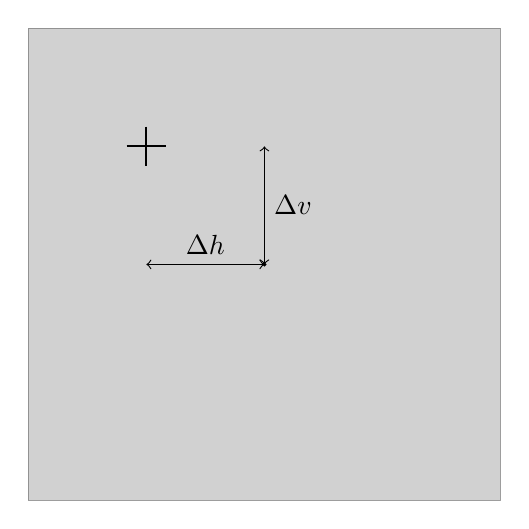
\begin{tikzpicture}
            \draw[fill=black!60!white,opacity=0.3] (-3, 3) -- (3, 3) -- (3, -3) -- (-3, -3) -- (-3, 3);
            \draw[fill=black] (0,0) circle (0.5pt);

            % Verschiebung
            \draw[thick] (-1.75, 1.5) -- (-1.25, 1.5);
            \draw[thick] (-1.5, 1.75) -- (-1.5, 1.25);

            % Pfeile & Beschriftung
            \draw[<->] (0, 1.5) -- (0, 0) node[pos=0.5,right] {$\Delta v$};
            \draw[<->] (0, 0) -- (-1.5, 0) node[pos=0.5,above] {$\Delta h$};
        \end{tikzpicture}
        \caption{Verschiebungsgeometrie}
        \label{fig:off_geometrie}
    \end{minipage}
\end{figure}

\subsubsection{Verschiebungen}\label{sssec:offset}

In einem idealen Modell sind die Strahlungsquelle und der Detektor genau aufeinander ausgerichtet, das heißt, dass der
Mittelpunkt der Strahlungsquelle und der Mittelpunkt des Detektors auf derselben Achse liegen. Durch den mechanischen
Aufbau einer realen Computertomographie-Anlage und deren händischer Justierung kommt es allerdings zu sowohl
einer horizontalen Verschiebung $\Delta h$ als auch einer vertikalen Verschiebung $\Delta v$ dieser Achse (siehe
Abbildung~\ref{fig:off_geometrie}). Von der Strahlungsquelle ausgehend trifft sie somit nicht mehr auf das Zentrum des
Detektors, sondern auf einen anderen Teil. Nimmt man Bezug auf die Detektorgeometrie, so müssen diese Verschiebungen
entsprechend berücksichtigt werden, da ansonsten ein verfälschtes Ergebnis berechnet wird. Dazu müssen die
Formeln~\ref{eq:det_h} und~\ref{eq:det_v} wie folgt umgeschrieben werden:

\begin{equation} 
    h_{min} + \frac{N_h \cdot d_h}{2} + \Delta h = 0
\end{equation}

\begin{equation}
    v_{min} + \frac{N_v \cdot d_v}{2}  + \Delta v = 0
\end{equation}

\subsubsection{Fehlende Projektionen}

Es leuchtet ein, dass Projektionen, die im Abstand von 180 Grad aufgenommen wurden, das durchleuchtete Objekt
spiegelverkehrt darstellen. In der Theorie würde es also ausreichen, einen Halbkreis um das Objekt abzufahren, um alle
erforderlichen Informationen für die Rückprojektion zu gewinnen. In der Praxis kann es aufgrund mechanischer Fehler bei
der Rotation des Quelle-Detektor-Aufbaus allerdings dazu kommen, dass einzelne Projektionen übersprungen werden oder die
Winkelabstände zwischen zwei Projektionen verschieden groß sind. Das Abfahren eines Vollkreises dient dazu, die so
entstandenen Fehler durch Redundanzen zu minimieren.

\subsection{Geometrische Berechnungen}\label{ssec:geometrie}

\subsubsection{Volumengeometrie}\label{sssec:vol_geometrie}

Für die Berechnung der Rückprojektion ist notwendig, die Zahl der im Volumen enthaltenen \gls{voxel} sowie deren
physische Ausdehnungen zu kennen. Da diese Informationen als Eingabeparameter des \gls{fdk} nicht zur Verfügung stehen,
müssen sie aus den bekannten geometrischen Parametern errechnet werden.

Betrachtet man die Abbildung~\ref{fig:fdk_geometrie}, so stellt man fest, dass zwischen den Volumendimensionen $x_k$ und
$y_l$ sowie der Detektordimension $h$ ein Zusammenhang besteht.

Die geschilderten Zusammenhänge sind für die Volumendimension $z_m$ und die Detektordimension $v$ äquivalent, sodass
sich die gezeigten Formeln durch den Austausch der relevanten Parameter auf diese übertragen lassen.

\subsubsection{Physische und nichtphysische Koordinatensysteme}\label{sssec:phys_coord}

Die in Abschnitt~\ref{ssec:fdk} vorgestellten Formeln zur Wichtung, Filterung und Rückprojektion setzen voraus, dass
sich die Ursprünge der Volumen- und Detektorkoordinatensysteme in den Zentren der zugehörigen Objekte befinden. Der für
die mathematische Betrachtung der Rückprojektion vernünftige Ansatz führt jedoch zu Problemen, wenn es um die
Adressierung des Speichers geht. Das erste Element eines reservierten Speicherbereichs mit $n$ Elementen hat stets den
Index $0$, das Zentrum den Index $\frac{n - 1}{2}$. Übertragen auf das Volumenkoordinatensystem heißt das, dass der
Ursprung mit den \textit{physischen} Koordinaten $(0, 0, 0)$ in einem dreidimensionalen Speicherbereich an der Stelle
$(\frac{x - 1}{2}, \frac{y - 1}{2}, \frac{z - 1}{2})$ zu finden ist, wobei $x$, $y$ und $z$ die Zahl der Voxel in der
jeweiligen Dimension angeben. Um die Formeln also bei der Implementierung der Rückprojektion nutzen zu können, ist eine
Umrechnung in das jeweils andere Koordinatensystem erforderlich.

Die Umrechnung eines Speicherindexes in eine physische Adresse lässt sich leicht durchführen. Ausgehend von $V$
Elementen in einer beliebigen Dimension, die jeweils $d_v$ Millimeter breit sind, lässt sich die physische Größe $V'$
des durch den Speicherbereich abgebildeten Objekts und damit auch dessen physischer Mittelpunkt $V'_M$ in dieser
Dimension bestimmen:

\begin{equation}
    \begin{aligned}
        V' &= V \cdot d_v\\
        V'_M &= \frac{V'}{2}
    \end{aligned}
\end{equation}

Stellt man sich die Elemente in horizontaler Anordnung vor und weist dem äußerst linken Element den Index $0$, also den
Ursprung, zu, so lässt sich über die Multiplikation des Indexes mit $d_v$ die physische Grenze (Kante) zwischen zwei
Elementen bestimmen. Der linke Rand des ersten Elements befindet sich also bei $0$ mm, die Kante zwischen dem ersten und
dem zweiten Element bei $d_v$ mm, zwischen dem zweiten und dritten Element bei $2 \cdot d_v$ mm usw. Durch die
Verschiebung des Ursprungs auf $V'_M$ ergibt sich nun das Problem, dass dieser nun für ungerade $V$ im Mittelpunkt eines
Elements liegt, für gerade $V$ dagegen auf der Kante zwischen zwei Elementen. Es ist deswegen sinnvoll, die physische
Koordinate $v'$ des Elements mit dem Index $v$ durch den Abstand des Elementzentrums vom Ursprung zu bestimmen:

\begin{equation}\label{eq:mem_to_phys}
    v' = -V_M' + \frac{d_v}{2} + v \cdot d_v
\end{equation}

Die Formel~\ref{eq:mem_to_phys} stellt die Umrechnung eines Indexes im Speicher in eine physische Koordinate dar. Durch
die Anwendung dieser Formel auf jede betrachtete Dimension ($x$, $y$ und $z$ für das Volumen, $h$ und $v$ für den
Detektor) lässt sich diese Umrechnung auch im Raum bzw.\ in der Ebene durchführen. Durch die Umstellung der Formel nach
$v$ lässt sich auch der umgekehrte Weg gehen.

Bei der Anwendung auf das Detektorkoordinatensystem sind die in Abschnitt~\ref{sssec:offset} genannten Verschiebungen zu
beachten. Exemplarisch wird diese Berücksichtung in Formel~\ref{eq:phys_to_mem} gezeigt, die die Umrechnung einer
der physischen Koordinate $p'$ in einen Speicherindex $p$ darstellt, wobei $P_M'$ dem physischen Mittelpunkt der
\gls{pixel} in dieser Dimension entspricht, $d_p$ deren physischer Breite und $\Delta p$ der Verschiebung:

\begin{equation}\label{eq:phys_to_mem}
    p = \frac{p' + P_M' + \Delta p}{d_p} - \frac{1}{2}
\end{equation}

Die Implementierung dieser Formeln mit \gls{cuda} ist den angehängten Quelltexten~\ref{app:coord_vol}
und~\ref{app:coord_det} zu entnehmen.

\subsection{Implementierung der Vorstufen}

Bevor die Rückprojektion erfolgen kann, müssen die individuellen Projektionen gewichtet und gefiltert werden. Die
Implementierung mit \gls{cuda} wird in den folgenden beiden Abschnitten beschrieben.

\subsubsection{Wichtung}

Die Grundlage der Wichtungsoperation ist die in Abschnitt~\ref{sssec:fdk_wichtung} vorgestellte
Formel~\ref{eq:wichtung}:

\begin{equation*}
    w_{ij} = \frac{d_{det} - d_{src}}{\sqrt{(d_{det} - d_{src})^2 + h_j^2 + v_i^2}}
\end{equation*}

Es ist leicht zu sehen, dass sich der Wichtungsfaktor $w_{ij}$ zwar pro \gls{pixel} ändert, aber nicht von der konkreten
Projektion abhängig ist. Es ist daher möglich, die Berechnung der Wichtungsfaktoren am Anfang des Programms genau einmal
durchzuführen und in einer Wichtungsmatrix \texttt{m} zu speichern (siehe Quelltext~\ref{source:impl_gen_mat}). Die
Berechnung der Wichtungsmatrix hängt von mehreren geometrischen Parametern ab (vgl.\
Abschnitt~\ref{sssec:fdk_geometrie} und Abbildungen~\ref{fig:det_geometrie},~\ref{fig:det_pixel},~\ref{fig:det_koord},~\ref{fig:off_geometrie}):

\begin{itemize}
    \item \texttt{dim\_x}: Anzahl der \gls{pixel} in horizontaler Richtung. Entspricht der Anzahl der Detektorpixel in
          horizontaler Richtung $N_h$
    \item \texttt{dim\_y}: Anzahl der \gls{pixel} in vertikaler Richtung. Entspricht der Anzahl der Detektorpixel in
          vertikaler Richtung $N_v$
    \item \texttt{h\_min}: horizontaler Abstand vom Detektorrand zum Detektorzentrum in mm.
    \item \texttt{v\_min}: vertikaler Abstand vom Detektorrand zum Detektorzentrum in mm.
    \item \texttt{d\_sd}: Abstand von der Quelle zum Detektor. Entsprich der Differenz der Strecken $d_{det}$ (Abstand
          zwischen dem Objekt und dem Detektor) und $d_{src}$ (Abstand zwischen der Quelle und dem Objekt) bzw.\ der
          Summe ihrer Beträge:
          
          \begin{equation*}
              d_{det} - d_{src} = |d_{det}| + |d_{src}|
          \end{equation*}

    \item \texttt{l\_px\_row}: horizontale Länge eines \gls{pixel}s, also der horizontale Abstand zwischen den
          Mittelpunkten zweier aufeinanderfolgender \gls{pixel}. Entspricht der horizontalen Länge eines Detektorpixels
          $d_h$.
    \item \texttt{l\_px\_col}: vertikale Länge eines \gls{pixel}s, also der vertikale Abstand zwischen den
          Mittelpunkten zweier aufeinanderfolgender \gls{pixel}. Entspricht der vertikalen Länge eines Detektorpixels
          $d_v$.
\end{itemize}

\begin{code}
\begin{minted}[breaklines,breakafter=\,,escapeinside=||,fontsize=\small]{cuda}
__global__ void matrix_generation_kernel(float* m,
    std::uint32_t dim_x, std::uint32_t dim_y, std::size_t pitch,
    float h_min, float v_min, float d_sd, float l_px_row,
    float l_px_col)
{
    auto s = blockIdx.x * blockDim.x + threadIdx.x;
    auto t = blockIdx.y * blockDim.y + threadIdx.y;

    if((s < dim_x) && (t < dim_y))
    {
        auto row = |\textbf{\textcolor{keyword-green}{reinterpret\_cast}}|<float*>(
            |\textbf{\textcolor{keyword-green}{reinterpret\_cast}}|<char*>(m) + t * pitch);

        // Detektorkoordinaten in mm
        const auto h_s = (l_px_row / 2.f) + s * l_px_row + h_min;
        const auto v_t = (l_px_col / 2.f) + t * l_px_col + v_min;

        // berechne Wichtungsfaktor
        row[s] = d_sd * rsqrtf(d_sd * d_sd + h_s * h_s + v_t * v_t);
    }
}
\end{minted}
\captionof{listing}{Generierung der Wichtungsmatrix}
\label{source:impl_gen_mat}
\end{code}

Bei der Wichtung einer Projektion \texttt{p} kann der jeweilige Wichtungsfaktor aus der generierten Matrix \texttt{m}
ausgelesen und auf das zugehörige \gls{pixel} angewendet werden (siehe Quelltext~\ref{source:impl_weighting}). 

\begin{code}
\begin{minted}[breaklines,breakafter=\,,escapeinside=||,fontsize=\small]{cuda}
__global__ void weighting_kernel(float* p, const float* m,
    std::uint32_t dim_x, std::uint32_t dim_y, std::size_t pitch,
    std::size_t m_pitch)
{
    auto s = blockIdx.x * blockDim.x + threadIdx.x;
    auto t = blockIdx.y * blockDim.y + threadIdx.y;

    if((s < dim_x) && (t < dim_y))
    {
        auto p_row = |\textbf{\textcolor{keyword-green}{reinterpret\_cast}}|<float*>(
            |\textbf{\textcolor{keyword-green}{reinterpret\_cast}}|<char*>(p) + t * pitch);
        auto m_row = |\textbf{\textcolor{keyword-green}{reinterpret\_cast}}|<const float*>(
            |\textbf{\textcolor{keyword-green}{reinterpret\_cast}}|<const char*>(m) + t * m_pitch);

        // Wichtung
        p_row[s] *= m_row[s];
    }
}
\end{minted}
\captionof{listing}{Wichtung einer Projektion}
\label{source:impl_weighting}
\end{code}

\subsubsection{Filterung}

Dem in Abschnitt~\ref{sssec:fdk_filter} vorgestellten Algorithmus entsprechend, folgt die Implementierung des
Filterschrittes dem nachstehenden Schema:

\begin{enumerate}
    \item einmalige Erzeugung und Fouriertransformation des Filters
    \item zeilenweise Fouriertransformation der Projektion
    \item Anwendung des Filters auf die jeweilige Projektionszeile im komplexen Raum
    \item inverse zeilenweise Fouriertransformation der Projektion
\end{enumerate}

Die Implementierung der Filtergenerierung entspricht der Formel~\ref{eq:filter_gen} und kann dem im Anhang befindlichen
Quelltext~\ref{app:filter_gen} entnommen werden. Dieser Filter wird dann zeilenweise auf jede Projektion angewendet.
Dazu werden der Filter und die einzelnen Projektionszeilen mit der \gls{cufft}-Bibliothek zunächst fouriertransformiert.
Im komplexen Raum werden dann die einzelnen Elemente der transformierten Projektionszeile mit den korrespondierenden
Elementen des transformierten Filters multipliziert (siehe Quelltext~\ref{source:impl_filter}). Ist dieser Vorgang
abgeschlossen, wird die Projektion wieder zurücktransformiert und normalisiert (siehe den angehängten
Quelltext~\ref{app:filter_norm}). Die Projektion ist dann bereit für die Rückprojektion.

\begin{code}
\begin{minted}[breaklines,breakafter=\,,escapeinside=||,fontsize=\small]{cuda}
__global__ void filter_application_kernel(
    cufftComplex* __restrict__ data,
    const cufftComplex* __restrict__ filter,
    std::uint32_t filter_size, std::uint32_t data_height,
    std::size_t pitch)
{
    auto x = blockIdx.x * blockDim.x + threadIdx.x;
    auto y = blockIdx.y * blockDim.y + threadIdx.y;

    if((x < filter_size) && (y < data_height))
    {
        auto row = |\textbf{\textcolor{keyword-green}{reinterpret\_cast}}|<cufftComplex*>(
            |\textbf{\textcolor{keyword-green}{reinterpret\_cast}}|<char*>(data) + y * pitch);

        row[x].x *= filter[x].x;
        row[x].y *= filter[x].y;
    }
}
\end{minted}
\captionof{listing}{Filterung einer Projektion}
\label{source:impl_filter}
\end{code}

\subsection{Implementierung der gefilterten Rückprojektion}

Die Implementierung der gefilterten Rückprojektion soll möglichst optimal auf der \gls{gpu} laufen. Um dies zu
erreichen, sind drei Dinge erforderlich: eine hohe Auslastung, geringe Wartezeiten zwischen den Rückprojektionen
der individuellen Projektionen und möglichst schnelle Zugriffe auf den globalen Speicher.

Eine hohe Auslastung der \gls{gpu} für einen gegebenen \gls{kernel}, also die gleichzeitige Ausführung einer hohen
Anzahl von Threads, ist dann möglich, wenn jeder Thread sehr wenige geteilte Ressourcen für seine Ausführung benötigt.
Bei diesen Ressourcen handelt es sich vor allem um die Register und den \textit{shared memory}, die pro \gls{sm} und
nicht pro Kern vorhanden sind.

Der Registerverbrauch eines \gls{kernel}s ist vor allem von zwei Faktoren abhängig: der Zahl der an den \gls{kernel}
übergebenen Funktionsparameter sowie der Zahl der lokalen Variablen pro Thread, die beispielsweise zur Speicherung der
Zwischenergebnisse benötigt werden. Die Minimierung beider Zahlen führt daher zu einem geringeren Registerverbrauch und
somit zu einer effizienteren Verteilung und Ausführung der Threads auf den Multiprozessoren. Da ein großer Teil der
Berechnungen auf der Detektorgeometrie aufbaut (siehe Abbildung~\ref{fig:fdk_geometrie}) und diese für alle Projektionen
unverändert bleibt, ist ein großer Teil der Parameter konstant. Indem man diese Konstanten nicht als Parameter übergibt,
sondern im konstanten Speicher (siehe Abschnitt~\ref{sssec:cu_mem}) der Grafikkarte ablegt, können einige Register
eingespart werden, sodass nur die in Quelltext~\ref{source:fdk_kernel_param} gezeigten Parameter übrig bleiben. Die
Struktur der konstanten Parameter wird in Quelltext~\ref{app:fdk_consts} gezeigt.

\begin{code}
\begin{minted}[breaklines,breakafter=\,,fontsize=\small]{cuda}
__global__ void backprojection_kernel(
    float* vol,                 // Zeiger auf das Volumen
    std::size_t vol_pitch,      // Volumen-Pitch
    cudaTextureObject_t proj,   // in Textur umgewandelte Projektion
    float angle_sin,            // Sinus des Projektionswinkels
    float angle_cos)            // Kosinus des Projektionswinkels
{
    /* ... */
}
\end{minted}
\caption{FDK-\gls{kernel}-Deklaration}
\label{source:fdk_kernel_param}
\end{code}

Schwieriger ist die Reduzierung der lokalen Variablen, die zur Speicherung von Zwischenergebnissen verwendet werden. Da
jeder Thread ein \gls{voxel} bearbeitet und jedes \gls{voxel} je eine Koordinate in $x$-, $y$- und $z$-Richtung besitzt,
sind wenigstens drei Variablen zur Speicherung dieser Koordinaten erforderlich. Hinzu kommen die von den
\gls{voxel}-Koordinaten abhängigen weiteren Variablen, wie etwa die beiden zugehörigen Projektionskoordinaten ($h$ und
$v$ im Projektionskoordinatensystem). Die Zwischenergebnisse erfüllen zudem einen bestimmten Zweck -- eine Entfernung
der zugehörigen Variablen führt daher an anderer Stelle zu unübersichtlicherem Quelltext, da die Berechnungen dennoch
durchgeführt werden müssen. Von einer manuellen Optimierung des Einsatzes lokaler Variablen ist aus diesen Gründen daher
abzusehen; es erscheint sinnvoller, sich auf die im Compiler vorhandenen automatischen Algorithmen zur Optimierung zu
verlassen.

Jeder Thread arbeitet auf einem bestimmten \gls{voxel} und ist zu dessen Berechnung nicht auf benachbarte Threads
angewiesen. Darüber hinaus ist dieses \gls{voxel} von genau einer Lese- und genau einer Schreiboperation betroffen. Der
Einsatz von \textit{shared memory} bietet daher für die Rückprojektion keinen Mehrwert.

Die Minimierung der Wartezeiten wird, wie in Abschnitt~\ref{ssec:loesungsvorschlag} erwähnt, durch die Ausführung der
Rückprojektion in einem eigenen Thread und Stream erreicht. Die im Hauptthread gewichteten und gefilterten Projektionen
werden in einer Warteschlange abgelegt und aus dieser nach dem FIFO-Prinzip vom Rückprojektionsthread entnommen. Der
Rückprojektions-\gls{kernel} wird dann mit der entnommenen Projektion gestartet und in den Rückprojektions-Stream
eingereiht.

Ein weiterer Faktor, der die Ausführungszeit beeinflusst, ist der Zugriff auf den globalen Speicher, in welchem sich
das Volumen und die Projektionen befinden. Die Projektionen müssen in diesem Schritt nicht mehr verändert werden und
sind daher konstant. Aufgrund ihrer Datengröße, die üblicherweise mehrere Megabyte beträgt, sind sie für den konstanten
Speicher zu groß. Es ist aber möglich, sie in eine \gls{cuda}-Textur umzuwandeln, um so von den auf der \gls{gpu}
verbauten Textur-Caches Gebrauch zu machen. Diese sind insbesondere dann effizient, wenn häufig auf benachbarte
\gls{pixel} zugegriffen werden muss. Für die Zwecke der Rückprojektion ist das ideal, da benachbarte Threads auf
benachbarten \gls{voxel}n arbeiten und benachbarte \gls{voxel} wiederum auf benachbarte \gls{pixel} projiziert werden.
Die \gls{cuda}-Texturroutinen bieten außerdem den Vorteil, dass eine lineare Interpolation beim Zugriff auf die
\gls{pixel} direkt ausgeführt werden kann -- diese Funktion muss also nicht selbst implementiert werden, was einerseits
die Komplexität des Quelltextes verringert und andererseits den von NVIDIA{\textregistered} optimierten Weg nutzt.

Auf das Volumen selbst erfolgen lesende und schreibende Zugriffe, eine Verwendung von \gls{cuda}-Texturen ist hier daher
nicht möglich. Da man sich innerhalb des Volumens im dreidimensionalen Raum bewegt, ist es sinnvoll, den für das Volumen
benötigten globalen Speicher so zu reservieren, dass dreidimensionale Zugriffe optimal erfolgen können. Die in
\gls{cuda} enthaltene Funktion \texttt{cudaMalloc3D} führt so eine Reservierung durch (vgl.
Abschnitt~\ref{sssec:cu_mem}). Die Zuordnung eines Threads zu einem bestimmten Punkt innerhalb des Datenfeldes erfolgt
auf ähnliche Weise wie bei einem zweidimensionalem Feld, nur dass hier noch die jeweilige Schicht des Volumens ermittelt
werden muss, wie in Quelltext~\ref{source:vol_slice_row} dargestellt.

\begin{code}
\begin{minted}[breaklines,breakafter=\,,escapeinside=||,fontsize=\small]{cuda}
    auto k = blockIdx.x * blockDim.x + threadIdx.x;
    auto l = blockIdx.y * blockDim.y + threadIdx.y;
    auto m = blockIdx.z * blockDim.z + threadIdx.z;

    if((k < consts.vol_dim_x) && (l < consts.vol_dim_y) &&
       (z < consts.vol_dim_z))
    {
        auto slice_pitch = vol_pitch * consts.vol_dim_y;
        auto slice = |\textbf{\textcolor{keyword-green}{reinterpret\_cast}}|<char*>(vol) + m * slice_pitch;
        auto row = |\textbf{\textcolor{keyword-green}{reinterpret\_cast}}|<float*>(slice + l * vol_pitch);
        /* ... */
    }    
\end{minted}
\caption{Zuordnung eines Threads zu einer Schicht und einer Zeile in der Schicht}
\label{source:vol_slice_row}
\end{code}

Da der vorherige Wert des Voxels zum jeweils aktuellen Wert hinzu addiert wird -- am Anfang haben alle Voxel des
Volumens den Wert 0 --, muss dieser vor der Addition aus dem globalen Speicher geladen werden. Trotz der bereits
getroffenen Optimierungen ist dieser Zugriff immer noch mit einer hohen Latenzzeit verbunden, die allerdings maskiert
werden kann. Zu diesem Zweck lädt man den alten Wert schon zu Beginn des \gls{kernel}s aus dem Speicher, sodass
Berechnungen, die von diesem Wert unabhängig sind, während der Wartezeit ausgeführt werden können (siehe
Quelltext~\ref{source:fdk_old_val}).

\begin{code}
\begin{minted}[breaklines,breakafter=\,,fontsize=\small]{cuda}
        auto old_val = row[k];
\end{minted}
\caption{\textit{Prefetch} des vorherigen Voxelwertes}
\label{source:fdk_old_val}
\end{code}

Die Berechnung der Rückprojektion erfolgt mittels der in Abschnitt~\ref{sssec:backprojection} vorgestellten Formeln. Der
Implementierung liegt dabei die in Abbildung~\ref{fig:fdk_geometrie} gezeigte Geometrie zugrunde. Zunächst ist ein
Wechsel des Koordinatensystems nötig, wie er in Quelltext~\ref{source:vol_coord_switch} zu sehen ist, da das Voxel
$(0, 0, 0)$ des im Speicher gehaltenen Volumens in einer der Volumenecken liegt, die Berechnungsvorschriften dagegen von
einem Ursprung ausgehen, der sich im Zentrum des Volumens befindet. Die Umrechnung einer Voxelkoordinate in eine
physische Koordinate wurde in Abschnitt~\ref{ssec:geometrie} beschrieben.

\begin{code}
\begin{minted}[breaklines,breakafter=\,,fontsize=\small]{cuda}
        auto x_k = vol_centered_coordinate(k, consts.vol_dim_x,
                                           consts.l_vx_x);
        auto y_l = vol_centered_coordinate(l, consts.vol_dim_y,
                                           consts.l_vx_y);
        auto z_m = vol_centered_coordinate(m, consts.vol_dim_z,
                                           consts.l_vx_z);
\end{minted}
\caption{Wechsel des Volumenkoordinatensystems}
\label{source:vol_coord_switch}
\end{code}

Die ermittelten physischen Volumenkoordinaten werden dann unter Berücksichtigung des Aufnahmewinkels der jeweiligen
Projektion auf den Detektor projiziert (siehe Quelltext~\ref{source:vol_coord_rot}). Analog zum Vorgehen bei der
Bestimmung der physischen Volumenkoordinaten müssen die physischen Projektionskoordinaten für den Zugriff auf das
Projektionsdatenfeld wieder in Pixelkoordinaten umgerechnet werden, sodass der Punkt $(0, 0)$ in der oberen linken Ecke
der Projektion liegt.

\begin{code}
\begin{minted}[breaklines,breakafter=\,,fontsize=\small]{cuda}
        // Koordinaten rotieren
        auto s = x_k * angle_cos + y_l * angle_sin;
        auto t = -x_k * angle_sin + y_l * angle_cos;

        // projizierte Koordinaten auf Detektor
        auto factor = consts.d_sd / (s + consts.d_so);
        auto h = proj_pixel_coordinate(t * factor, consts.proj_dim_x,
             consts.l_px_x, consts.delta_s) + 0.5f;
        auto v = proj_pixel_coordinate(z_m * factor,
             consts.proj_dim_y, consts.l_px_y, consts.delta_t) + 0.5f;
\end{minted}
\caption{Projektion der Volumenkoordinaten auf den Detektor}
\label{source:vol_coord_rot}
\end{code}

An der Stelle $(h, v)$ kann jetzt der Pixelwert ermittelt bzw.\ linear interpoliert und dann für die in
Quelltext~\ref{source:vol_bp} dargestellte Rückprojektion herangezogen werden. Erst an diesem Punkt kommt der zu Beginn
des \gls{kernel}s geladene vorherige Voxelwert zum Einsatz, dessen Ladezeit durch die vorangegangenen Berechnungen
maskiert wurde.

\begin{code}
\begin{minted}[breaklines,breakafter=\,,fontsize=\small]{cuda}
        // Projektionswert interpolieren
        auto det = tex2D<float>(proj, h, v);

        // Rückprojektion
        auto u = -(consts.d_so / (s + consts.d_so));
        row[k] = old_val + 0.5f * det * u * u;
\end{minted}
\caption{Detektorinterpolation und Rückprojektion}
\label{source:vol_bp}
\end{code}

Der vollständige Rückprojektions-\gls{kernel} findet sich in Anhang~\ref{app:impl_bp}. Aufgerufen wird der beschriebene
\gls{kernel} für jede Projektion einzeln. Durch die Aneinanderreihung der einzelnen \gls{kernel}-Instanzen im selben
Stream wird sichergestellt, dass niemals zwei Rückprojektionen gleichzeitig auf einem \gls{device} ausgeführt werden,
sodass weitere Synchronisierungsmechanismen nicht erforderlich sind.
